\subsection*{Redigering}
Redigering inddeles i en boundary og en tilhørende controller, som det fremgår af \autoref{fig:Redigering}. 

\begin{figure} [H]
\centering
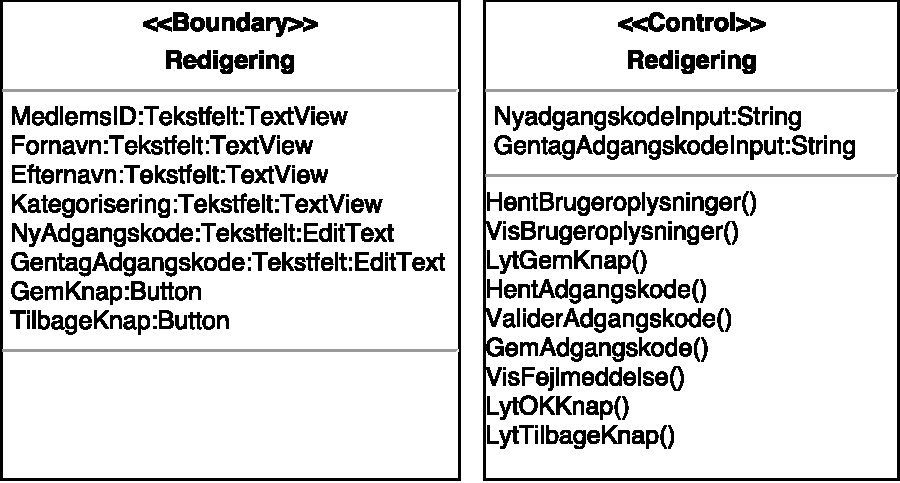
\includegraphics[width=0.9\textwidth]{figures/MVC/Redigering}
\caption{Designklasser for Redigering. Til venstre fremgår boundary og til højre controller for redigering.}
\label{fig:Redigering}
\end{figure}

\noindent
I grænsefladen for \textit{redigering} opstilles tekstfelter af typen TextView for medlemsID, fornavn, efternavn og kategorisering. Derudover opstilles tekstfelter, af typen EditText, for ny adgangskode og gentag adgangskode, hvor brugeren kan ændre adgangskoden. Dertil er der en GemKnap og en TilbageKnap, af typen Button. Gemknappen indikerer ved tryk, at brugeren ønsker at gemme den nye adgangskode. 
Den tilhørende controller har metoderne Hent, Vis, Lyt, Valider og Gem. Til disse klasser er der opstillet et sekvensdiagram, hvilket fremgår af \autoref{fig:SEKRedigering}.


\begin{figure} [H]
\centering
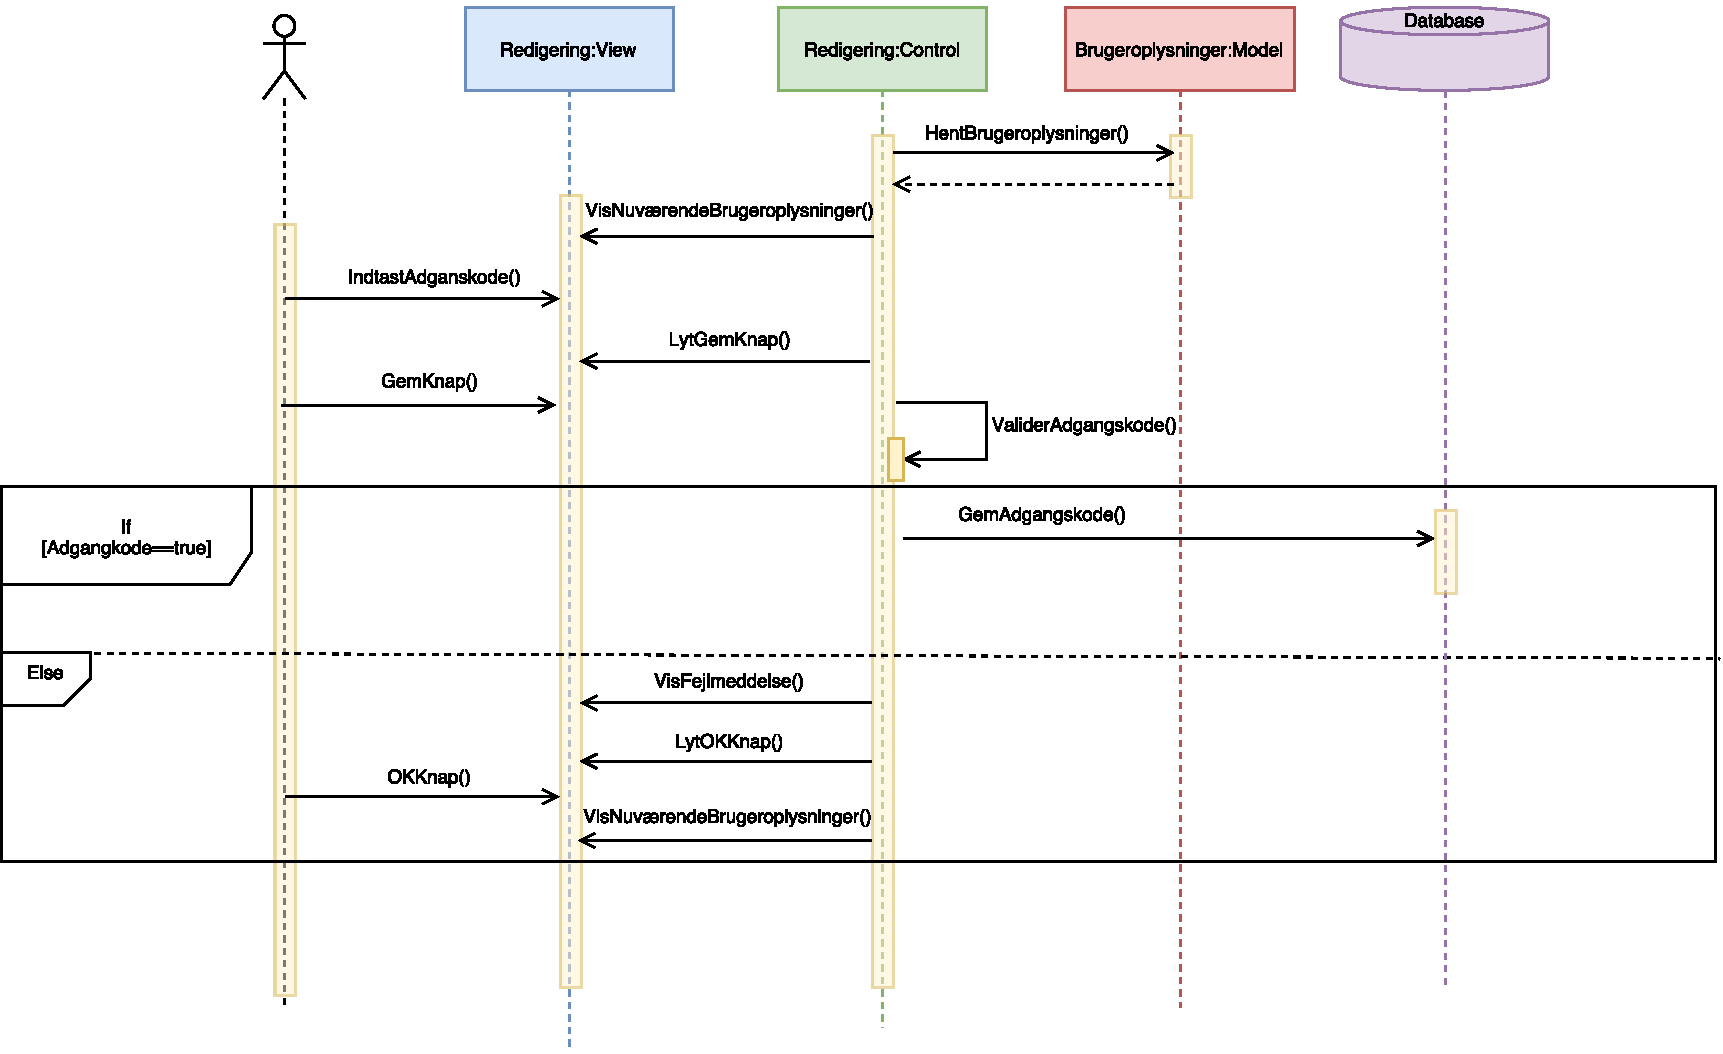
\includegraphics[width=1.4\textwidth, angle=90]{figures/Sek/SEKRedigering}
\caption{Sekvensdiagram for redigering.}
\label{fig:SEKRedigering}
\end{figure}

\noindent
Controlleren \textit{Redigering} henter brugeroplysninger fra modellen \textit{Brugeroplysninger}. Disse oplysninger vises i grænsefladen \textit{Redigering}, hvortil brugeren kan se deres information. Fra denne grænseflade er det ligeledes muligt for brugeren at ændre sin adgangskode. Adgangskoden skal indtastes to gange for at sikre, at adgangskoden er identisk. Dertil skal adgangskoden være minimum 10 karakterer lang. Adgangskoden valideres, hvis adgangskoden overholder de førnævnte kriterier og gemmes direkte i databasen. Dette gøres af sikkerhedsmæssige årsager, således koden ikke først gemmes, idet brugeren logger ud af app'en. 
Overholder adgangskoden derimod ikke kriterierne, vises en grænseflade for fejlmeddelelse. På denne grænseflade er der opstillet en OKKnap, der ved tryk henviser systemet tilbage til grænsefladen for redigering. 
